%%%%%%%%%%%%%%%%%%%%%%%%%%%%%%%%%%%%%%%%%
% Data Collections Summary
% LaTeX Template
% Version 2.1 (1/10/15)
%
% This template has been downloaded from:
% http://www.LaTeXTemplates.com
%
% Original author:
% Mathias Legrand (legrand.mathias@gmail.com) 
% With extensive modifications by:
% Vel (vel@latextemplates.com)
%
% License:
% CC BY-NC-SA 3.0 (http://creativecommons.org/licenses/by-nc-sa/3.0/)
%
%%%%%%%%%%%%%%%%%%%%%%%%%%%%%%%%%%%%%%%%%

%----------------------------------------------------------------------------------------
%	PACKAGES AND OTHER DOCUMENT CONFIGURATIONS
%----------------------------------------------------------------------------------------

\documentclass[obeyspaces, spaces, fleqn,10pt]{SelfArx} % Document font size and equations flushed left

\usepackage[english]{babel} % Specify a different language here - english by default

\usepackage{lipsum} % Required to insert dummy text. To be removed otherwise

\PassOptionsToPackage{obeyspaces, spaces}{url}
\usepackage[obeyspaces, spaces]{url}
\usepackage{minted}
\def\UrlBreaks{\do\/\do-}

%----------------------------------------------------------------------------------------
%	COLUMNS
%----------------------------------------------------------------------------------------

\setlength{\columnsep}{0.55cm} % Distance between the two columns of text
\setlength{\fboxrule}{0.75pt} % Width of the border around the abstract

%----------------------------------------------------------------------------------------
%	COLORS
%----------------------------------------------------------------------------------------

\definecolor{color1}{RGB}{0,0,0} % Color of the article title and sections
\definecolor{color2}{RGB}{53 88,118} % Color of the boxes behind the abstract and headings

%----------------------------------------------------------------------------------------
%	HYPERLINKS
%----------------------------------------------------------------------------------------

\usepackage{hyperref} % Required for hyperlinks
\hypersetup{hidelinks,colorlinks,breaklinks=true,urlcolor=color2,citecolor=color1,linkcolor=color1,bookmarksopen=false,pdftitle={Title},pdfauthor={Author}}

%----------------------------------------------------------------------------------------
%	ARTICLE INFORMATION
%----------------------------------------------------------------------------------------

\Archive{May 12, 2019} % Additional notes (e.g. copyright, DOI, review/research article)
\JournalInfo{Data Science 2: CS109B} % Journal information

\PaperTitle{Algorithmic Biases in Facial Recognition} % Article title

\Authors{Whitney Jablonski, Paul Jureidini, Samata Kurhekar, Shourya Veeraganti} % Authors
%\affiliation{\textsuperscript{1}\textit{Department of Biology, University of Examples, London, United Kingdom}} % Author affiliation
%\affiliation{\textsuperscript{2}\textit{Department of Chemistry, University of Examples, London, United Kingdom}} % Author affiliation
%\affiliation{*\textbf{Corresponding author}: john@smith.com} % Corresponding author

\Keywords{} % Keywords - if you don't want any simply remove all the text between the curly brackets
%\newcommand{\keywordname}{Keywords} % Defines the keywords heading name

%----------------------------------------------------------------------------------------
%	ABSTRACT
%----------------------------------------------------------------------------------------

%\Abstract{}

%----------------------------------------------------------------------------------------

\begin{document}

\flushbottom % Makes all text pages the same height

\maketitle % Print the title and abstract box

\tableofcontents % Print the contents section

\thispagestyle{empty} % Removes page numbering from the first page

%----------------------------------------------------------------------------------------
%	ARTICLE CONTENTS
%----------------------------------------------------------------------------------------

\section*{Summary} % The \section*{} command stops section numbering

\addcontentsline{toc}{section}{Summary} % Adds this section to the table of contents

%\lipsum[1-3] % Dummy text
% and some mathematics $\cos\pi=-1$ and $\alpha$ in the text\footnote{And some mathematics $\cos\pi=-1$ and $\alpha$ in the text.}.

Add in the summary when results section is finished.

%------------------------------------------------

\section{Introduction}

Facial analysis and facial recognition are technologies fueled by artificial intelligence that are becoming more entrenched in our every day lives even in a broad range of areas. Applications range from smartphone cameras (e.g., auto-focusing), law enforcement (e.g., border security, risk assessment for recidivism), and advertisement targeting (e.g., from profile pictures).\cite{Couch:2017,Lohr:2018,Kim:2018} The crux of the issue lies in the insufficiently diverse training data sets that introduce bias into machine learning algorithms used in all of the applications listed. Popular, publicly available, and easily accessible data sets such as Labeled Faces in the Wild (LFW) are used by software companies (e.g., Google) for benchmarking their facial recognition machine learning algorithms.\cite{LFWTech,Lohr:2018} In 2015, Google's facial recognition app mistakenly identified black people as gorillas which kicked off a conversation about algorithmic bias and its potential implications for humans.\cite{dough2015,Lohr:2018} Algorithmic bias like that which caused the misidentification of black people can be introduced during training when using data sets such as LFW which Wang et. al. estimated to be nearly 85\% white.\cite{wang:2018}  The resulting model will inherently have more error in identifying underrepresented races, and therefore the algorithm will more accurately predict features of better represented races. 

In this work, we evaluate racial algorithmic bias from the standpoint of gender classification using several publicly available data sets. First, we discuss the selection process for the data set and features of the data, the models used herein, and our choice for using gender classification as a benchmark. Then we detail our approach for image pre-processing, data ingestion to the mode, the model architecture, and augmentation of images for model improvement. Finally, we present a comparison of the performance for gender classification with respect to race for each of the methods outlined. Our overarching goal is to reduce algorithmic bias by training a convolutional neural net (CNN) for gender classification using a more diverse training data set, and then test it against an existing non-diverse training data set (e.g., LFW).

\subsection{Image Data Selection}
A summary of four publicly available facial image databases that we evaluated for this study is given in Table \ref{tab:tab1}. For our purposes, we sought a data set with explicit labels for race and gender. The VGGFace2 data set is the most comprehensive with over 3.3 million faces and more than 8600 identities at different ages.\cite{Cao18} Unfortunately, VGGFace2 is not explicitly labeled for race, and therefore we opted to use the UTKFace data set which was conveniently labeled for both gender and race with a relatively good sample size of 23,000 images.\cite{utkface} We evaluated LFW and a data set created by a group in China called 'Racial Faces in the Wild' with race labels, but neither data set suited our needs for gender labels.\cite{LFWTech,wang:2018} 

\begin{table}[hbt]
\caption{Summary of facial image databases.}
\centering
\begin{tabular}{lclc}
\toprule
%\multicolumn{2}{c}{Name} \\
%\cmidrule(r){1-2}
Name & \# Faces (thousands) & Labels & Ref \\
\midrule
VGGFace2 & ~3,300 & a,g,i & \cite{Cao18} \\
LFW & 13 & i & \cite{LFWTech} \\
RFW & 665 & r,i & \cite{wang:2018} \\
UTKFace & 23 & a,g,r & \cite{utkface} \\
\bottomrule
\multicolumn{4}{l}{age (a), gender (g), race (r), identity (i)} \\
\end{tabular}
\label{tab:tab1}
\end{table}

The UTKFace data was developed by researchers at the University of Tennessee Knoxville (UTK) who were developing a conditional adversarial autoencoder for age progression/regression and sought a racially and age-balanced data set.\cite{utkface} As a result, there is a wide range of ages of the people represented in the images. UTKFace contains images that range in age from 1 to 116 with a mean age of 33. Four races and one aggregated category are represented: white, black, asian, indian, and other (hispanic, latino, middle eastern). A comparison of the distribution for age and race with respect to gender is shown in Figure \ref{fig:fig2}. Male and female are represented fairly equally among the races with slightly more male images in the white and indian categories and slightly more female images in the asian and other categories. We are not explicitly dealing with age for our analysis, but we anecdotally observe that male images between ages 20 to 60 are more evenly distributed whereas there are far more female images between ages 20 and 40. For our analysis, we limit the range of ages to between age 10 to 65. 

\begin{figure}[ht]\centering % Using \begin{figure*} makes the figure take up the entire width of the page
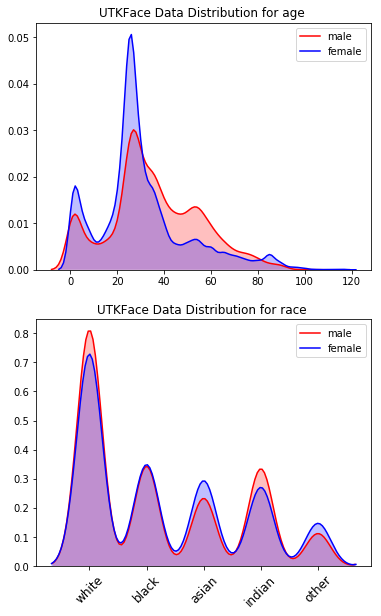
\includegraphics[width=\linewidth]{img/UTKfaces_age-gender-distribution}
\caption{Age and race distribution in the UTKFace data set with respect to the gender.}
\label{fig:fig2}
\end{figure}

The UTKFace data set is available in 2 formats: either "in-the-wild" wherein faces are not explicitly cropped and aligned but contain a single face per image or aligned and cropped to a single face. There are readily available software packages that aid in face detection, image alignment, and cropping and therefore we will not discuss those techniques.\cite{dlib09,mtcnn} To accommodate our compressed time frame and to allow us to explore more interesting aspects of model development and fine-tuning, we will use the cropped and aligned UTKFace data set. Eight randomly chosen images from that data set are shown in Figure \ref{fig:fig1} along with their corresponding age, race, and gender labels at the top of the image. In this subset of images and in general, the labels appear to be correctly assigned for the most part. We did not rigorously evaluate each of the images to verify the labels, but we performed a cursory visual inspection of a few hundred images and found the labels to be correct in more than 95\% of the cases.

\begin{figure*}[ht]\centering % Using \begin{figure*} makes the figure take up the entire width of the page
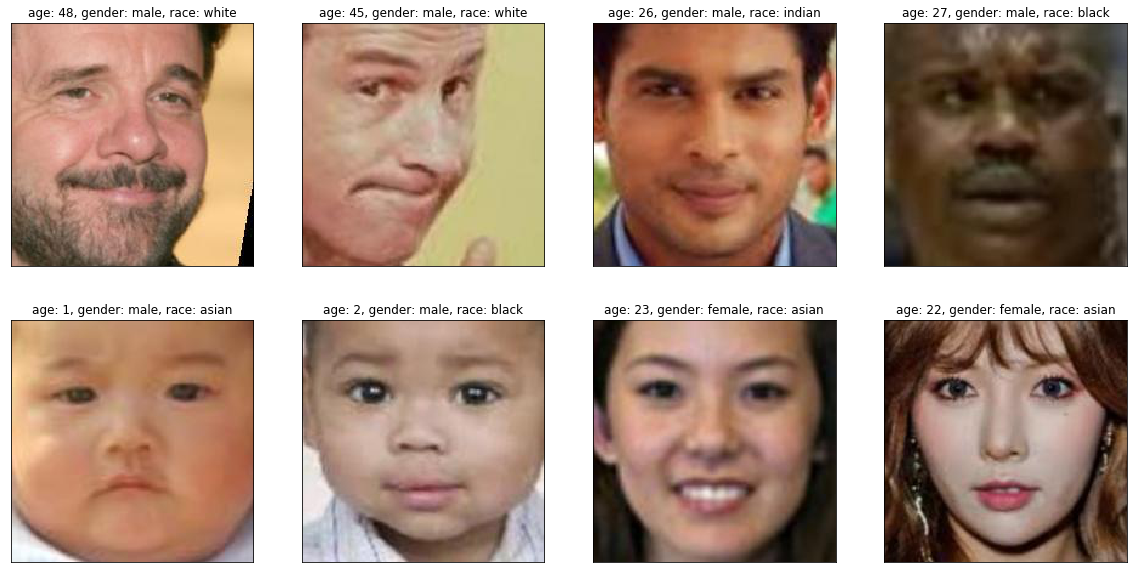
\includegraphics[width=\linewidth]{img/UTKfaces_labelverification}
\caption{A random sampling of images plotted with their labels shows that the UTKFace data set has very accurate labeling.}
\label{fig:fig1}
\end{figure*}

\subsection{Model Selection}
We evaluated several publicly available facial recognition models in the hopes of leveraging them with transfer learning to build our gender classifier. Transfer learning is a nuanced practice, and for our purposes we define it as using pre-trained weights and/or the general architecture of an existing model using similar data to perform a new classification task.\cite{brownlee:transfer,sarkar} A comparison of model complexity in terms of the number of parameters for each model is given in Table \ref{tab:tab2}. 

\begin{table}[hbt]
\caption{Summary of transfer learning models.}
\centering
\begin{tabular}{lclc}
\toprule
%\multicolumn{2}{c}{Name} \\
%\cmidrule(r){1-2}
Model & \# Parameters (million) & Ref \\
\midrule
VGG & 138 & \cite{Simonyan14c} \\
InceptionV3 & 7 & \cite{inceptionv3} \\
ResNet50 & 25.5 & \cite{resnet} \\
\bottomrule
\end{tabular}
\label{tab:tab2}
\end{table}

\noindent Each of the models listed in Table \ref{tab:tab2} are available with pre-trained weights for identity classification. For our purposes, we intend to use a neural network model for the classification of gender in a racially diverse data set. Because none of these models are trained for binary classification of gender, we found that they did not do well in classifying gender out-of-the-box. When the models listed in Table \ref{tab:tab2}, one can either use the full model directly or use only the architecture and trainimag using a different data set. Prior to training, the architecture can be manipulated to perform a new task (e.g., gender classification) or to achieve higher accuracy for different data sets. 

The models listed in Table \ref{tab:tab2} are highly complex with millions of parameters each. We decided to evaluate a much simpler model to juxtapose the possibility that a small architecture tuned with a balanced data set can achieve good accuracy for gender classification. Subedi recently developed a CNN with 674,178 parameters for gender, age, and race classification from the UTKFace data set, and the architecture is shown in Figure \ref{fig:fig3}.\cite{subedi} Subedi's model architecture consists of 5 2D convolution layers each with a batch normalization layer followed by a 2D maximum pooling layer afterwards. The input layer uses a filter size of 32, and each subsequent convolutional layer multiplies the filter size by an integer corresponding to the layer number (e.g., for concolutional layer 2 the filter size is 32 $\times$ 2). The activation function is a rectified linear unit (ReLU) for all convolutional layers. Subedi uses a so-called 'bottleneck' layer (\mintinline{python}{GlobalMaxPool2D} in Keras) which outputs a 1-dimensional tensor and feeds 3 separate dense layers to produce 3 outputs. In this way, a dense layer is defined for each of the 3 categories each with an appropriate activation function for the type of classification problem (e.g., binary or multiclass). When the model is created, the 3 dense layers are passed in a list as the output. For our purposes, we have adapted the model to output only the gender classification.

\begin{figure*}[ht]\centering % Using \begin{figure*} makes the figure take up the entire width of the page
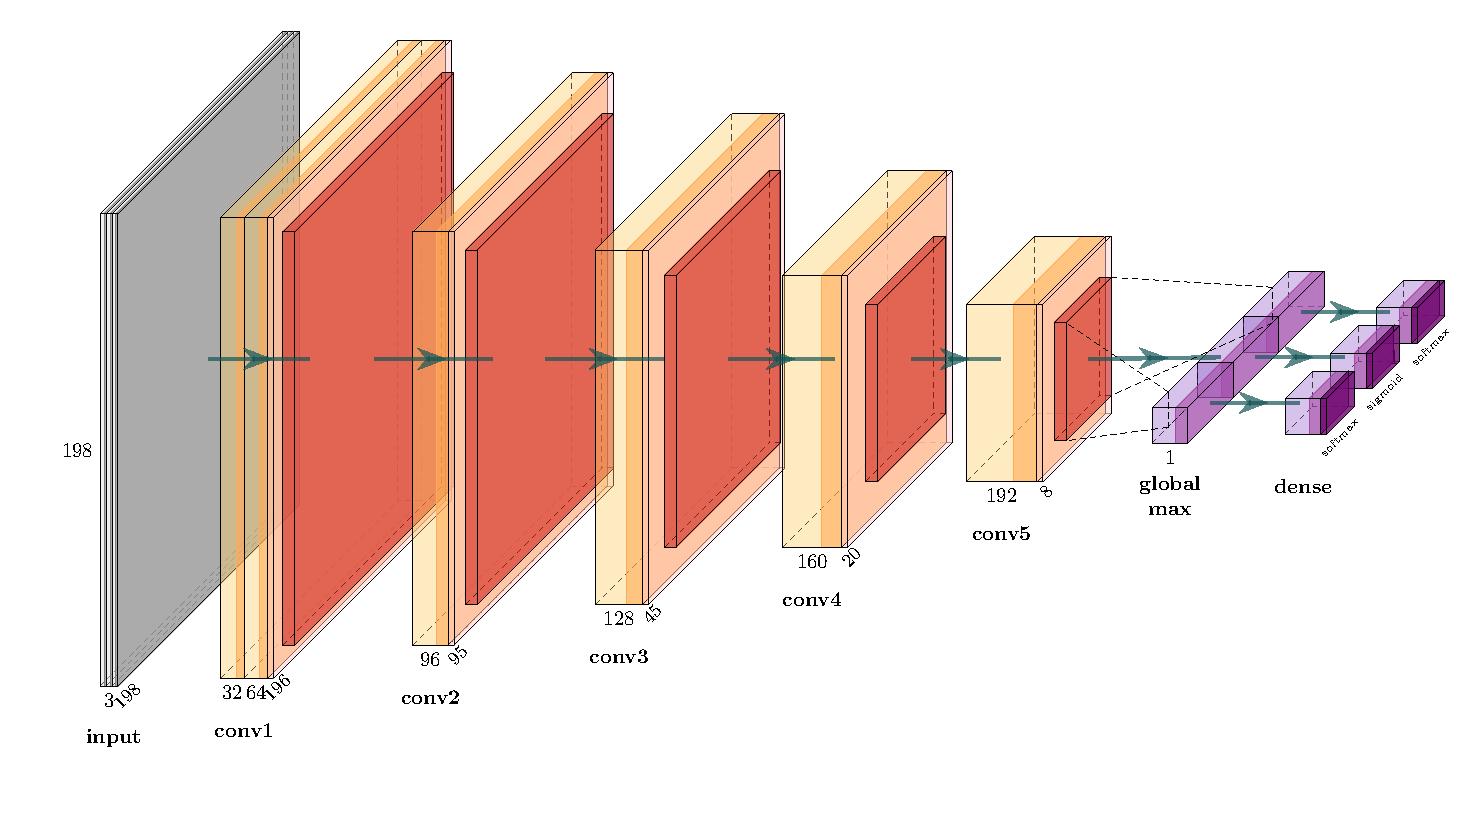
\includegraphics[width=\linewidth]{img/subedi}
\caption{Architecture of neural network developed by Subedi for age, gender, and race classification.}
\label{fig:fig3}
\end{figure*}

\begin{figure*}[hp]\centering % Using \begin{figure*} makes the figure take up the entire width of the page
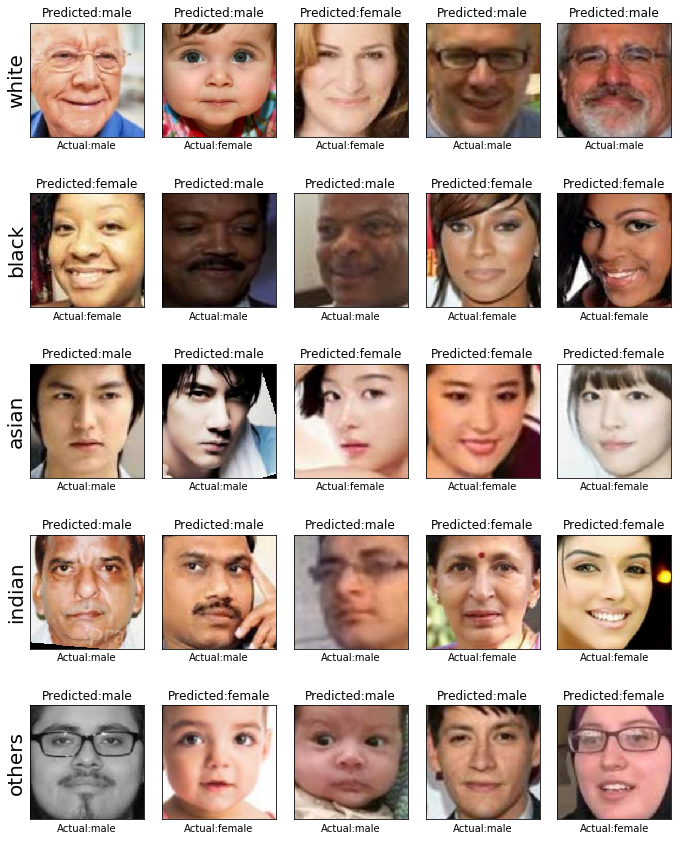
\includegraphics[width=.95\linewidth]{img/base-case-model-results}
\caption{Base case model results with classification results as the top caption and the ground truth as the bottom caption.}
\label{fig:fig4}
\end{figure*}

%------------------------------------------------

\section{Methodology}

Keras with a GPU Tensorflow back end was used for implementing and evaluating CNNs, and all models were run using an NVIDIA Tesla K80 GPU. All code written and used from other sources for this report is given in the accompanying iPython Notebook. 

\subsection{Image Preprocessing}

Data ingestion into the model is not straightforward for large data sets, and can create a bottleneck for feeding the neural network that can cause undesirably high computational times. The goal for any data generator is to leverage all available system resources for ingesting data efficiently so that the bottleneck for computation is not the process of feeding data into the model.\cite{amidi} Keras has a built-in \mintinline{python}{ImageDataGenerator} class, and we evaluated this for some of the models. Generally, though, we found that results were more comprehensible and predictable using our own custom generator based on the one that was developed by Subedi. We found this uniquely useful when applied with UTKFace data because of the relatively small size of the training data set and the CNN. This allowed us to use a simple data generator that takes in image filenames from a data frame and delivers batches of a user-specified size directly to the model through \mintinline{python}{fit_generator}. 

\subsection{Image Augmentation}

One drawback to using a custom data generator is that we could not leverage the convenient functions available in the call to Keras' \mintinline{python}{ImageDataGenerator} for image augementation. As such, we built functionality into our custom generator to add random noise and flip images within the data set as it is ingested into the model. We used the \mintinline{python}{augmenters} class from within the \mintinline{python}{imgaug} package to sequentially augment images by adding black pixels to 2\% of the image (\mintinline{python}{CoarseDropout}) and then flipping the image.  Model was overfitting when flipping only 30\% of the data. When we changed the flip proportion to 50\% then the model performed better. 

We used over-sampling and down-sampling to balance the data set. The 'other' race had the fewest images (1153) in the training data, and we 'down-sampled' the number of images for the other races to include the same number of images. Over-sampling was done by matching the number of images in the race with the most images (white, 6755). Images of races with fewer than 6755 images were added to the training data set by sampling with replacement. The new over-sampled training data set was then passed via the image data generator to the model. Through that pipeline, the image augmentation wrapped inside the data generator ensured that no two images were identical. 

%------------------------------------------------

\section{Results}

Because we began with a broad range of models and data for this work, we began by performing cursory experiments with each model to evaluate 1) computational time, 2) baseline accuracy, and 3) ease of use. Our initial results made it clear that working with the pre-trained models would be computationally prohibitive. We also found that they did not achieve satisfactory results for gender classification. 

\subsection{Gender Classification with Racially Diverse}
Performance with respect to age



Used 16 filters 
\lipsum[11] % Dummy text

\subsection{Training with Races Balanced}

We took two approaches to balancing the data set: over-sampling and down-sampling. 
\lipsum[11] % Dummy text


\lipsum[11] % Dummy text
\subsection{Feature Representation Mapping}
\lipsum[11] % Dummy text


saliency map
discuss how PCA might be used to evaluate features for determining gender, but it's beyond the scope of this project. You might use PCA 

\subsection{Validation with Other Data Sets}
We validated the model using the VGGFace2 and the RFW test data sets. 
\lipsum[11] % Dummy text

confusion matrix

\section{Conclusions}
During this project we improved a classifier for gender prediction from racially heterogeneous images. Our accomplishments include:


\begin{itemize}
\item list of conclusions
\item list of conclusions
\item list of conclusions
\end{itemize}
%------------------------------------------------
\phantomsection

%----------------------------------------------------------------------------------------
%	REFERENCE LIST
%----------------------------------------------------------------------------------------
\phantomsection
\Urlmuskip=0mu plus 2mu\relax
\bibliographystyle{unsrt}
\bibliography{references}

%----------------------------------------------------------------------------------------

\end{document}